\documentclass[1p]{elsarticle_modified}
%\bibliographystyle{elsarticle-num}

%\usepackage[colorlinks]{hyperref}
%\usepackage{abbrmath_seonhwa} %\Abb, \Ascr, \Acal ,\Abf, \Afrak
\usepackage{amsfonts}
\usepackage{amssymb}
\usepackage{amsmath}
\usepackage{amsthm}
\usepackage{scalefnt}
\usepackage{amsbsy}
\usepackage{kotex}
\usepackage{caption}
\usepackage{subfig}
\usepackage{color}
\usepackage{graphicx}
\usepackage{xcolor} %% white, black, red, green, blue, cyan, magenta, yellow
\usepackage{float}
\usepackage{setspace}
\usepackage{hyperref}

\usepackage{tikz}
\usetikzlibrary{arrows}

\usepackage{multirow}
\usepackage{array} % fixed length table
\usepackage{hhline}

%%%%%%%%%%%%%%%%%%%%%
\makeatletter
\renewcommand*\env@matrix[1][\arraystretch]{%
	\edef\arraystretch{#1}%
	\hskip -\arraycolsep
	\let\@ifnextchar\new@ifnextchar
	\array{*\c@MaxMatrixCols c}}
\makeatother %https://tex.stackexchange.com/questions/14071/how-can-i-increase-the-line-spacing-in-a-matrix
%%%%%%%%%%%%%%%

\usepackage[normalem]{ulem}

\newcommand{\msout}[1]{\ifmmode\text{\sout{\ensuremath{#1}}}\else\sout{#1}\fi}
%SOURCE: \msout is \stkout macro in https://tex.stackexchange.com/questions/20609/strikeout-in-math-mode

\newcommand{\cancel}[1]{
	\ifmmode
	{\color{red}\msout{#1}}
	\else
	{\color{red}\sout{#1}}
	\fi
}

\newcommand{\add}[1]{
	{\color{blue}\uwave{#1}}
}

\newcommand{\replace}[2]{
	\ifmmode
	{\color{red}\msout{#1}}{\color{blue}\uwave{#2}}
	\else
	{\color{red}\sout{#1}}{\color{blue}\uwave{#2}}
	\fi
}

\newcommand{\Sol}{\mathcal{S}} %segment
\newcommand{\D}{D} %diagram
\newcommand{\A}{\mathcal{A}} %arc


%%%%%%%%%%%%%%%%%%%%%%%%%%%%%5 test

\def\sl{\operatorname{\textup{SL}}(2,\Cbb)}
\def\psl{\operatorname{\textup{PSL}}(2,\Cbb)}
\def\quan{\mkern 1mu \triangleright \mkern 1mu}

\theoremstyle{definition}
\newtheorem{thm}{Theorem}[section]
\newtheorem{prop}[thm]{Proposition}
\newtheorem{lem}[thm]{Lemma}
\newtheorem{ques}[thm]{Question}
\newtheorem{cor}[thm]{Corollary}
\newtheorem{defn}[thm]{Definition}
\newtheorem{exam}[thm]{Example}
\newtheorem{rmk}[thm]{Remark}
\newtheorem{alg}[thm]{Algorithm}

\newcommand{\I}{\sqrt{-1}}
\begin{document}

%\begin{frontmatter}
%
%\title{Boundary parabolic representations of knots up to 8 crossings}
%
%%% Group authors per affiliation:
%\author{Yunhi Cho} 
%\address{Department of Mathematics, University of Seoul, Seoul, Korea}
%\ead{yhcho@uos.ac.kr}
%
%
%\author{Seonhwa Kim} %\fnref{s_kim}}
%\address{Center for Geometry and Physics, Institute for Basic Science, Pohang, 37673, Korea}
%\ead{ryeona17@ibs.re.kr}
%
%\author{Hyuk Kim}
%\address{Department of Mathematical Sciences, Seoul National University, Seoul 08826, Korea}
%\ead{hyukkim@snu.ac.kr}
%
%\author{Seokbeom Yoon}
%\address{Department of Mathematical Sciences, Seoul National University, Seoul, 08826,  Korea}
%\ead{sbyoon15@snu.ac.kr}
%
%\begin{abstract}
%We find all boundary parabolic representation of knots up to 8 crossings.
%
%\end{abstract}
%\begin{keyword}
%    \MSC[2010] 57M25 
%\end{keyword}
%
%\end{frontmatter}

%\linenumbers
%\tableofcontents
%
\newcommand\colored[1]{\textcolor{white}{\rule[-0.35ex]{0.8em}{1.4ex}}\kern-0.8em\color{red} #1}%
%\newcommand\colored[1]{\textcolor{white}{ #1}\kern-2.17ex	\textcolor{white}{ #1}\kern-1.81ex	\textcolor{white}{ #1}\kern-2.15ex\color{red}#1	}

{\Large $\underline{12a_{1010}~(K12a_{1010})}$}

\setlength{\tabcolsep}{10pt}
\renewcommand{\arraystretch}{1.6}
\vspace{1cm}\begin{tabular}{m{100pt}>{\centering\arraybackslash}m{274pt}}
\multirow{5}{120pt}{
	\centering
	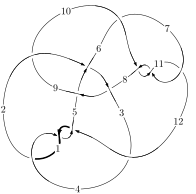
\includegraphics[width=112pt]{../../../GIT/diagram.site/Diagrams/png/1811_12a_1010.png}\\
\ \ \ A knot diagram\footnotemark}&
\allowdisplaybreaks
\textbf{Linearized knot diagam} \\
\cline{2-2}
 &
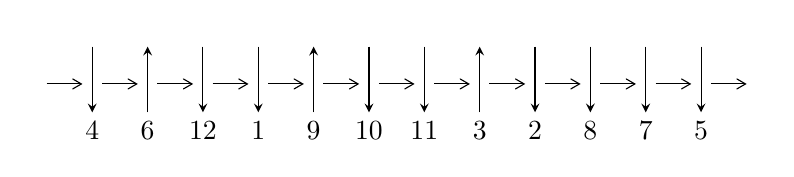
\begin{tikzpicture}[x=20pt, y=17pt]
	% nodes
	\node (C0) at (0, 0) {};
	\node (C1) at (1, 0) {};
	\node (C1U) at (1, +1) {};
	\node (C1D) at (1, -1) {4};

	\node (C2) at (2, 0) {};
	\node (C2U) at (2, +1) {};
	\node (C2D) at (2, -1) {6};

	\node (C3) at (3, 0) {};
	\node (C3U) at (3, +1) {};
	\node (C3D) at (3, -1) {12};

	\node (C4) at (4, 0) {};
	\node (C4U) at (4, +1) {};
	\node (C4D) at (4, -1) {1};

	\node (C5) at (5, 0) {};
	\node (C5U) at (5, +1) {};
	\node (C5D) at (5, -1) {9};

	\node (C6) at (6, 0) {};
	\node (C6U) at (6, +1) {};
	\node (C6D) at (6, -1) {10};

	\node (C7) at (7, 0) {};
	\node (C7U) at (7, +1) {};
	\node (C7D) at (7, -1) {11};

	\node (C8) at (8, 0) {};
	\node (C8U) at (8, +1) {};
	\node (C8D) at (8, -1) {3};

	\node (C9) at (9, 0) {};
	\node (C9U) at (9, +1) {};
	\node (C9D) at (9, -1) {2};

	\node (C10) at (10, 0) {};
	\node (C10U) at (10, +1) {};
	\node (C10D) at (10, -1) {8};

	\node (C11) at (11, 0) {};
	\node (C11U) at (11, +1) {};
	\node (C11D) at (11, -1) {7};

	\node (C12) at (12, 0) {};
	\node (C12U) at (12, +1) {};
	\node (C12D) at (12, -1) {5};
	\node (C13) at (13, 0) {};

	% arrows
	\draw[->,>={angle 60}]
	(C0) edge (C1) (C1) edge (C2) (C2) edge (C3) (C3) edge (C4) (C4) edge (C5) (C5) edge (C6) (C6) edge (C7) (C7) edge (C8) (C8) edge (C9) (C9) edge (C10) (C10) edge (C11) (C11) edge (C12) (C12) edge (C13) ;	\draw[->,>=stealth]
	(C1U) edge (C1D) (C2D) edge (C2U) (C3U) edge (C3D) (C4U) edge (C4D) (C5D) edge (C5U) (C6U) edge (C6D) (C7U) edge (C7D) (C8D) edge (C8U) (C9U) edge (C9D) (C10U) edge (C10D) (C11U) edge (C11D) (C12U) edge (C12D) ;
	\end{tikzpicture} \\
\hhline{~~} \\& 
\textbf{Solving Sequence} \\ \cline{2-2} 
 &
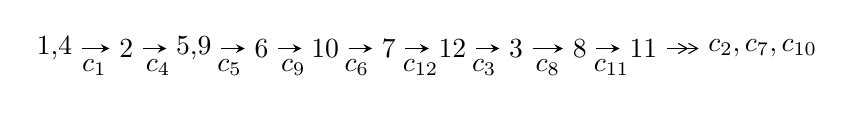
\begin{tikzpicture}[x=23pt, y=7pt]
	% node
	\node (A0) at (-1/8, 0) {1,4};
	\node (A1) at (1, 0) {2};
	\node (A2) at (33/16, 0) {5,9};
	\node (A3) at (25/8, 0) {6};
	\node (A4) at (33/8, 0) {10};
	\node (A5) at (41/8, 0) {7};
	\node (A6) at (49/8, 0) {12};
	\node (A7) at (57/8, 0) {3};
	\node (A8) at (65/8, 0) {8};
	\node (A9) at (73/8, 0) {11};
	\node (C1) at (1/2, -1) {$c_{1}$};
	\node (C2) at (3/2, -1) {$c_{4}$};
	\node (C3) at (21/8, -1) {$c_{5}$};
	\node (C4) at (29/8, -1) {$c_{9}$};
	\node (C5) at (37/8, -1) {$c_{6}$};
	\node (C6) at (45/8, -1) {$c_{12}$};
	\node (C7) at (53/8, -1) {$c_{3}$};
	\node (C8) at (61/8, -1) {$c_{8}$};
	\node (C9) at (69/8, -1) {$c_{11}$};
	\node (A10) at (11, 0) {$c_{2},c_{7},c_{10}$};

	% edge
	\draw[->,>=stealth]	
	(A0) edge (A1) (A1) edge (A2) (A2) edge (A3) (A3) edge (A4) (A4) edge (A5) (A5) edge (A6) (A6) edge (A7) (A7) edge (A8) (A8) edge (A9) ;
	\draw[->>,>={angle 60}]	
	(A9) edge (A10);
\end{tikzpicture} \\ 

\end{tabular} \\

\footnotetext{
The image of knot diagram is generated by the software ``\textbf{Draw programme}" developed by Andrew Bartholomew(\url{http://www.layer8.co.uk/maths/draw/index.htm\#Running-draw}), where we modified some parts for our purpose(\url{https://github.com/CATsTAILs/LinksPainter}).
}\phantom \\ \newline 
\centering \textbf{Ideals for irreducible components\footnotemark of $X_{\text{par}}$} 
 
\begin{align*}
I^u_{1}&=\langle 
- u^{11}-2 u^{10}-6 u^9-9 u^8-12 u^7-13 u^6-8 u^5-5 u^4+u^2+b,\\
\phantom{I^u_{1}}&\phantom{= \langle  }u^{11}+2 u^{10}+7 u^9+10 u^8+17 u^7+17 u^6+16 u^5+10 u^4+3 u^3+a-2 u-1,\\
\phantom{I^u_{1}}&\phantom{= \langle  }u^{13}+2 u^{12}+8 u^{11}+12 u^{10}+23 u^9+26 u^8+28 u^7+22 u^6+10 u^5+2 u^4-4 u^3-4 u^2- u-1\rangle \\
I^u_{2}&=\langle 
-1.77519\times10^{76} u^{83}+3.36042\times10^{76} u^{82}+\cdots+4.02015\times10^{76} b-3.79501\times10^{75},\\
\phantom{I^u_{2}}&\phantom{= \langle  }1.26819\times10^{76} u^{83}-1.95398\times10^{76} u^{82}+\cdots+4.02015\times10^{76} a-7.98274\times10^{76},\;u^{84}- u^{83}+\cdots-8 u+1\rangle \\
\\
\end{align*}
\raggedright * 2 irreducible components of $\dim_{\mathbb{C}}=0$, with total 97 representations.\\
\footnotetext{All coefficients of polynomials are rational numbers. But the coefficients are sometimes approximated in decimal forms when there is not enough margin.}
\newpage
\renewcommand{\arraystretch}{1}
\centering \section*{I. $I^u_{1}= \langle - u^{11}-2 u^{10}+\cdots+u^2+b,\;u^{11}+2 u^{10}+\cdots+a-1,\;u^{13}+2 u^{12}+\cdots- u-1 \rangle$}
\flushleft \textbf{(i) Arc colorings}\\
\begin{tabular}{m{7pt} m{180pt} m{7pt} m{180pt} }
\flushright $a_{1}=$&$\begin{pmatrix}1\\0\end{pmatrix}$ \\
\flushright $a_{4}=$&$\begin{pmatrix}0\\u\end{pmatrix}$ \\
\flushright $a_{2}=$&$\begin{pmatrix}1\\u^2\end{pmatrix}$ \\
\flushright $a_{5}=$&$\begin{pmatrix}- u\\u\end{pmatrix}$ \\
\flushright $a_{9}=$&$\begin{pmatrix}- u^{11}-2 u^{10}+\cdots+2 u+1\\u^{11}+2 u^{10}+6 u^9+9 u^8+12 u^7+13 u^6+8 u^5+5 u^4- u^2\end{pmatrix}$ \\
\flushright $a_{6}=$&$\begin{pmatrix}u^8+u^7+4 u^6+3 u^5+5 u^4+2 u^3+u^2- u-1\\- u^8- u^7-3 u^6-3 u^5-2 u^4-2 u^3+u^2+u\end{pmatrix}$ \\
\flushright $a_{10}=$&$\begin{pmatrix}- u^{11}-2 u^{10}+\cdots-2 u^2+u\\u^{11}+2 u^{10}+6 u^9+8 u^8+11 u^7+10 u^6+6 u^5+3 u^4- u^3-2 u^2\end{pmatrix}$ \\
\flushright $a_{7}=$&$\begin{pmatrix}u^{10}+2 u^9+7 u^8+10 u^7+16 u^6+16 u^5+13 u^4+8 u^3+u^2-1\\u^{12}+2 u^{11}+6 u^{10}+8 u^9+10 u^8+8 u^7+2 u^6-2 u^5-5 u^4-4 u^3\end{pmatrix}$ \\
\flushright $a_{12}=$&$\begin{pmatrix}u^2+1\\- u^2\end{pmatrix}$ \\
\flushright $a_{3}=$&$\begin{pmatrix}u^5+2 u^3+u\\- u^5- u^3+u\end{pmatrix}$ \\
\flushright $a_{8}=$&$\begin{pmatrix}- u^{12}-2 u^{11}+\cdots+u+1\\u^{12}+2 u^{11}+7 u^{10}+10 u^9+16 u^8+16 u^7+13 u^6+8 u^5+u^4- u^3- u^2- u\end{pmatrix}$ \\
\flushright $a_{11}=$&$\begin{pmatrix}- u^{11}-2 u^{10}+\cdots+u+1\\2 u^{11}+4 u^{10}+\cdots- u-1\end{pmatrix}$\\&\end{tabular}
\flushleft \textbf{(ii) Obstruction class $= -1$}\\~\\
\flushleft \textbf{(iii) Cusp Shapes $= 4 u^{12}+4 u^{11}+24 u^{10}+20 u^9+52 u^8+36 u^7+48 u^6+32 u^5+24 u^4+24 u^3+16 u^2+12 u+2$}\\~\\
\newpage\renewcommand{\arraystretch}{1}
\flushleft \textbf{(iv) u-Polynomials at the component}\newline \\
\begin{tabular}{m{50pt}|m{274pt}}
Crossings & \hspace{64pt}u-Polynomials at each crossing \\
\hline $$\begin{aligned}c_{1},c_{4},c_{7}\\c_{10},c_{11},c_{12}\end{aligned}$$&$\begin{aligned}
&u^{13}-2 u^{12}+\cdots- u+1
\end{aligned}$\\
\hline $$\begin{aligned}c_{2},c_{5}\end{aligned}$$&$\begin{aligned}
&u^{13}+2 u^{10}+7 u^9+10 u^6+12 u^5-8 u^4+4 u^3+4 u^2+u-1
\end{aligned}$\\
\hline $$\begin{aligned}c_{3},c_{6}\end{aligned}$$&$\begin{aligned}
&u^{13}+2 u^{12}+\cdots+5 u+2
\end{aligned}$\\
\hline $$\begin{aligned}c_{8}\end{aligned}$$&$\begin{aligned}
&u^{13}-19 u^{12}+\cdots+1856 u-256
\end{aligned}$\\
\hline $$\begin{aligned}c_{9}\end{aligned}$$&$\begin{aligned}
&u^{13}-19 u^{12}+\cdots+1344 u-192
\end{aligned}$\\
\hline
\end{tabular}\\~\\
\newpage\renewcommand{\arraystretch}{1}
\flushleft \textbf{(v) Riley Polynomials at the component}\newline \\
\begin{tabular}{m{50pt}|m{274pt}}
Crossings & \hspace{64pt}Riley Polynomials at each crossing \\
\hline $$\begin{aligned}c_{1},c_{4},c_{7}\\c_{10},c_{11},c_{12}\end{aligned}$$&$\begin{aligned}
&y^{13}+12 y^{12}+\cdots-7 y-1
\end{aligned}$\\
\hline $$\begin{aligned}c_{2},c_{5}\end{aligned}$$&$\begin{aligned}
&y^{13}+14 y^{11}+\cdots+9 y-1
\end{aligned}$\\
\hline $$\begin{aligned}c_{3},c_{6}\end{aligned}$$&$\begin{aligned}
&y^{13}-4 y^{12}+\cdots-39 y-4
\end{aligned}$\\
\hline $$\begin{aligned}c_{8}\end{aligned}$$&$\begin{aligned}
&y^{13}-35 y^{12}+\cdots+135168 y-65536
\end{aligned}$\\
\hline $$\begin{aligned}c_{9}\end{aligned}$$&$\begin{aligned}
&y^{13}-37 y^{12}+\cdots+49152 y-36864
\end{aligned}$\\
\hline
\end{tabular}\\~\\
\newpage\flushleft \textbf{(vi) Complex Volumes and Cusp Shapes}
$$\begin{array}{c|c|c}  
\text{Solutions to }I^u_{1}& \I (\text{vol} + \sqrt{-1}CS) & \text{Cusp shape}\\
 \hline 
\begin{aligned}
u &= -0.345201 + 1.021440 I \\
a &= \phantom{-}0.383027 + 0.071451 I \\
b &= \phantom{-}0.786816 + 0.242416 I\end{aligned}
 & -0.092600 - 0.790634 I & -5.74730 - 0.20798 I \\ \hline\begin{aligned}
u &= -0.345201 - 1.021440 I \\
a &= \phantom{-}0.383027 - 0.071451 I \\
b &= \phantom{-}0.786816 - 0.242416 I\end{aligned}
 & -0.092600 + 0.790634 I & -5.74730 + 0.20798 I \\ \hline\begin{aligned}
u &= -0.816966 + 0.218516 I \\
a &= -1.090410 - 0.648020 I \\
b &= \phantom{-}0.316522 - 0.929361 I\end{aligned}
 & -4.93693 + 9.42698 I & -10.17355 - 7.65318 I \\ \hline\begin{aligned}
u &= -0.816966 - 0.218516 I \\
a &= -1.090410 + 0.648020 I \\
b &= \phantom{-}0.316522 + 0.929361 I\end{aligned}
 & -4.93693 - 9.42698 I & -10.17355 + 7.65318 I \\ \hline\begin{aligned}
u &= \phantom{-}0.242549 + 1.320770 I \\
a &= \phantom{-}2.31317 + 2.33263 I \\
b &= -2.01116 - 2.58449 I\end{aligned}
 & \phantom{-}5.96169 - 6.15155 I & \phantom{-}2.5842 - 14.2195 I \\ \hline\begin{aligned}
u &= \phantom{-}0.242549 - 1.320770 I \\
a &= \phantom{-}2.31317 - 2.33263 I \\
b &= -2.01116 + 2.58449 I\end{aligned}
 & \phantom{-}5.96169 + 6.15155 I & \phantom{-}2.5842 + 14.2195 I \\ \hline\begin{aligned}
u &= \phantom{-}0.609274\phantom{ +0.000000I} \\
a &= -2.87003\phantom{ +0.000000I} \\
b &= \phantom{-}2.28717\phantom{ +0.000000I}\end{aligned}
 & -2.44873\phantom{ +0.000000I} & \phantom{-}31.6660\phantom{ +0.000000I} \\ \hline\begin{aligned}
u &= -0.08989 + 1.44411 I \\
a &= \phantom{-}0.86609 + 1.34154 I \\
b &= -1.31236 - 2.11003 I\end{aligned}
 & \phantom{-}13.07620 + 0.19322 I & \phantom{-}5.00344 + 0.65090 I \\ \hline\begin{aligned}
u &= -0.08989 - 1.44411 I \\
a &= \phantom{-}0.86609 - 1.34154 I \\
b &= -1.31236 + 2.11003 I\end{aligned}
 & \phantom{-}13.07620 - 0.19322 I & \phantom{-}5.00344 - 0.65090 I \\ \hline\begin{aligned}
u &= -0.34207 + 1.41123 I \\
a &= -0.20187 - 2.15080 I \\
b &= -0.37276 + 3.06306 I\end{aligned}
 & \phantom{-}5.4451 + 17.8321 I & -1.52643 - 9.77243 I\\
 \hline 
 \end{array}$$\newpage$$\begin{array}{c|c|c}  
\text{Solutions to }I^u_{1}& \I (\text{vol} + \sqrt{-1}CS) & \text{Cusp shape}\\
 \hline 
\begin{aligned}
u &= -0.34207 - 1.41123 I \\
a &= -0.20187 + 2.15080 I \\
b &= -0.37276 - 3.06306 I\end{aligned}
 & \phantom{-}5.4451 - 17.8321 I & -1.52643 + 9.77243 I \\ \hline\begin{aligned}
u &= \phantom{-}0.046940 + 0.495776 I \\
a &= \phantom{-}0.665010 + 1.116330 I \\
b &= \phantom{-}0.449357 + 0.078161 I\end{aligned}
 & \phantom{-}0.68765 - 1.39515 I & -0.97323 + 4.26024 I \\ \hline\begin{aligned}
u &= \phantom{-}0.046940 - 0.495776 I \\
a &= \phantom{-}0.665010 - 1.116330 I \\
b &= \phantom{-}0.449357 - 0.078161 I\end{aligned}
 & \phantom{-}0.68765 + 1.39515 I & -0.97323 - 4.26024 I\\
 \hline 
 \end{array}$$\newpage\newpage\renewcommand{\arraystretch}{1}
\centering \section*{II. $I^u_{2}= \langle -1.78\times10^{76} u^{83}+3.36\times10^{76} u^{82}+\cdots+4.02\times10^{76} b-3.80\times10^{75},\;1.27\times10^{76} u^{83}-1.95\times10^{76} u^{82}+\cdots+4.02\times10^{76} a-7.98\times10^{76},\;u^{84}- u^{83}+\cdots-8 u+1 \rangle$}
\flushleft \textbf{(i) Arc colorings}\\
\begin{tabular}{m{7pt} m{180pt} m{7pt} m{180pt} }
\flushright $a_{1}=$&$\begin{pmatrix}1\\0\end{pmatrix}$ \\
\flushright $a_{4}=$&$\begin{pmatrix}0\\u\end{pmatrix}$ \\
\flushright $a_{2}=$&$\begin{pmatrix}1\\u^2\end{pmatrix}$ \\
\flushright $a_{5}=$&$\begin{pmatrix}- u\\u\end{pmatrix}$ \\
\flushright $a_{9}=$&$\begin{pmatrix}-0.315458 u^{83}+0.486047 u^{82}+\cdots+5.80096 u+1.98568\\0.441574 u^{83}-0.835893 u^{82}+\cdots-5.12507 u+0.0943996\end{pmatrix}$ \\
\flushright $a_{6}=$&$\begin{pmatrix}0.789727 u^{83}-0.878458 u^{82}+\cdots+11.7409 u-0.991810\\0.518038 u^{83}-0.964879 u^{82}+\cdots-4.65016 u+0.772193\end{pmatrix}$ \\
\flushright $a_{10}=$&$\begin{pmatrix}-0.0980563 u^{83}+0.387555 u^{82}+\cdots+12.6062 u+1.72069\\0.0831270 u^{83}-0.0730730 u^{82}+\cdots-4.39119 u-0.0245108\end{pmatrix}$ \\
\flushright $a_{7}=$&$\begin{pmatrix}0.0825732 u^{83}+0.185608 u^{82}+\cdots-8.24132 u-0.987882\\0.241456 u^{83}-1.04811 u^{82}+\cdots+5.35494 u-0.163213\end{pmatrix}$ \\
\flushright $a_{12}=$&$\begin{pmatrix}u^2+1\\- u^2\end{pmatrix}$ \\
\flushright $a_{3}=$&$\begin{pmatrix}u^5+2 u^3+u\\- u^5- u^3+u\end{pmatrix}$ \\
\flushright $a_{8}=$&$\begin{pmatrix}-0.567135 u^{83}+0.694103 u^{82}+\cdots+11.9492 u+1.30203\\0.271257 u^{83}-0.00854034 u^{82}+\cdots-3.68237 u-0.132308\end{pmatrix}$ \\
\flushright $a_{11}=$&$\begin{pmatrix}-0.934228 u^{83}+0.597004 u^{82}+\cdots+6.80551 u+0.971587\\-0.0459951 u^{83}+0.774208 u^{82}+\cdots-3.42474 u+0.306200\end{pmatrix}$\\&\end{tabular}
\flushleft \textbf{(ii) Obstruction class $= -1$}\\~\\
\flushleft \textbf{(iii) Cusp Shapes $= -4.70327 u^{83}+5.21911 u^{82}+\cdots+16.9568 u-8.13028$}\\~\\
\newpage\renewcommand{\arraystretch}{1}
\flushleft \textbf{(iv) u-Polynomials at the component}\newline \\
\begin{tabular}{m{50pt}|m{274pt}}
Crossings & \hspace{64pt}u-Polynomials at each crossing \\
\hline $$\begin{aligned}c_{1},c_{4},c_{7}\\c_{10},c_{11},c_{12}\end{aligned}$$&$\begin{aligned}
&u^{84}+u^{83}+\cdots+8 u+1
\end{aligned}$\\
\hline $$\begin{aligned}c_{2},c_{5}\end{aligned}$$&$\begin{aligned}
&u^{84}-7 u^{83}+\cdots+8 u^2+1
\end{aligned}$\\
\hline $$\begin{aligned}c_{3},c_{6}\end{aligned}$$&$\begin{aligned}
&u^{84}- u^{83}+\cdots+124914 u+10897
\end{aligned}$\\
\hline $$\begin{aligned}c_{8}\end{aligned}$$&$\begin{aligned}
&(u^{42}+9 u^{41}+\cdots-19 u-1)^{2}
\end{aligned}$\\
\hline $$\begin{aligned}c_{9}\end{aligned}$$&$\begin{aligned}
&(u^{42}+8 u^{41}+\cdots+4 u-1)^{2}
\end{aligned}$\\
\hline
\end{tabular}\\~\\
\newpage\renewcommand{\arraystretch}{1}
\flushleft \textbf{(v) Riley Polynomials at the component}\newline \\
\begin{tabular}{m{50pt}|m{274pt}}
Crossings & \hspace{64pt}Riley Polynomials at each crossing \\
\hline $$\begin{aligned}c_{1},c_{4},c_{7}\\c_{10},c_{11},c_{12}\end{aligned}$$&$\begin{aligned}
&y^{84}+71 y^{83}+\cdots+392 y^2+1
\end{aligned}$\\
\hline $$\begin{aligned}c_{2},c_{5}\end{aligned}$$&$\begin{aligned}
&y^{84}+7 y^{83}+\cdots+16 y+1
\end{aligned}$\\
\hline $$\begin{aligned}c_{3},c_{6}\end{aligned}$$&$\begin{aligned}
&y^{84}-29 y^{83}+\cdots+1118832658 y+118744609
\end{aligned}$\\
\hline $$\begin{aligned}c_{8}\end{aligned}$$&$\begin{aligned}
&(y^{42}-29 y^{41}+\cdots-99 y+1)^{2}
\end{aligned}$\\
\hline $$\begin{aligned}c_{9}\end{aligned}$$&$\begin{aligned}
&(y^{42}-42 y^{41}+\cdots-64 y+1)^{2}
\end{aligned}$\\
\hline
\end{tabular}\\~\\
\newpage\flushleft \textbf{(vi) Complex Volumes and Cusp Shapes}
$$\begin{array}{c|c|c}  
\text{Solutions to }I^u_{2}& \I (\text{vol} + \sqrt{-1}CS) & \text{Cusp shape}\\
 \hline 
\begin{aligned}
u &= \phantom{-}0.518175 + 0.869909 I \\
a &= -0.038515 - 0.361398 I \\
b &= -0.396322 - 0.279186 I\end{aligned}
 & -2.21491 - 3.65443 I & \phantom{-0.000000 } 0 \\ \hline\begin{aligned}
u &= \phantom{-}0.518175 - 0.869909 I \\
a &= -0.038515 + 0.361398 I \\
b &= -0.396322 + 0.279186 I\end{aligned}
 & -2.21491 + 3.65443 I & \phantom{-0.000000 } 0 \\ \hline\begin{aligned}
u &= -0.486616 + 0.918991 I \\
a &= \phantom{-}0.669010 - 0.149675 I \\
b &= \phantom{-}0.548977 + 0.391483 I\end{aligned}
 & \phantom{-}2.27560 - 8.94034 I & \phantom{-0.000000 } 0 \\ \hline\begin{aligned}
u &= -0.486616 - 0.918991 I \\
a &= \phantom{-}0.669010 + 0.149675 I \\
b &= \phantom{-}0.548977 - 0.391483 I\end{aligned}
 & \phantom{-}2.27560 + 8.94034 I & \phantom{-0.000000 } 0 \\ \hline\begin{aligned}
u &= -0.433633 + 0.954309 I \\
a &= -0.568715 + 0.074268 I \\
b &= -0.630900 - 0.351516 I\end{aligned}
 & -2.64853 - 4.93654 I & \phantom{-0.000000 } 0 \\ \hline\begin{aligned}
u &= -0.433633 - 0.954309 I \\
a &= -0.568715 - 0.074268 I \\
b &= -0.630900 + 0.351516 I\end{aligned}
 & -2.64853 + 4.93654 I & \phantom{-0.000000 } 0 \\ \hline\begin{aligned}
u &= \phantom{-}0.874722 + 0.339102 I \\
a &= \phantom{-}0.230055 - 0.515951 I \\
b &= -0.327717 - 0.197359 I\end{aligned}
 & -0.08162 - 4.63366 I & \phantom{-0.000000 } 0 \\ \hline\begin{aligned}
u &= \phantom{-}0.874722 - 0.339102 I \\
a &= \phantom{-}0.230055 + 0.515951 I \\
b &= -0.327717 + 0.197359 I\end{aligned}
 & -0.08162 + 4.63366 I & \phantom{-0.000000 } 0 \\ \hline\begin{aligned}
u &= \phantom{-}0.922673 + 0.158839 I \\
a &= \phantom{-}0.134609 - 0.475277 I \\
b &= -0.171410 - 0.216206 I\end{aligned}
 & -0.40808 + 2.05165 I & \phantom{-0.000000 } 0 \\ \hline\begin{aligned}
u &= \phantom{-}0.922673 - 0.158839 I \\
a &= \phantom{-}0.134609 + 0.475277 I \\
b &= -0.171410 + 0.216206 I\end{aligned}
 & -0.40808 - 2.05165 I & \phantom{-0.000000 } 0\\
 \hline 
 \end{array}$$\newpage$$\begin{array}{c|c|c}  
\text{Solutions to }I^u_{2}& \I (\text{vol} + \sqrt{-1}CS) & \text{Cusp shape}\\
 \hline 
\begin{aligned}
u &= \phantom{-}0.875995 + 0.247622 I \\
a &= -0.202518 + 0.483595 I \\
b &= \phantom{-}0.264623 + 0.227684 I\end{aligned}
 & -4.19534 - 1.24503 I & -19.3254 + 4.7543 I \\ \hline\begin{aligned}
u &= \phantom{-}0.875995 - 0.247622 I \\
a &= -0.202518 - 0.483595 I \\
b &= \phantom{-}0.264623 - 0.227684 I\end{aligned}
 & -4.19534 + 1.24503 I & -19.3254 - 4.7543 I \\ \hline\begin{aligned}
u &= \phantom{-}0.589935 + 0.687179 I \\
a &= -0.092443 + 0.519015 I \\
b &= \phantom{-}0.441781 + 0.227681 I\end{aligned}
 & \phantom{-}1.163260 - 0.381253 I & -6.00000 + 5.04367 I \\ \hline\begin{aligned}
u &= \phantom{-}0.589935 - 0.687179 I \\
a &= -0.092443 - 0.519015 I \\
b &= \phantom{-}0.441781 - 0.227681 I\end{aligned}
 & \phantom{-}1.163260 + 0.381253 I & -6.00000 - 5.04367 I \\ \hline\begin{aligned}
u &= \phantom{-}0.542934 + 0.983292 I \\
a &= \phantom{-}0.024629 + 0.211855 I \\
b &= \phantom{-}0.392576 + 0.359601 I\end{aligned}
 & \phantom{-}2.14428 - 7.17345 I & \phantom{-0.000000 } 0 \\ \hline\begin{aligned}
u &= \phantom{-}0.542934 - 0.983292 I \\
a &= \phantom{-}0.024629 - 0.211855 I \\
b &= \phantom{-}0.392576 - 0.359601 I\end{aligned}
 & \phantom{-}2.14428 + 7.17345 I & \phantom{-0.000000 } 0 \\ \hline\begin{aligned}
u &= -0.829852 + 0.247067 I \\
a &= \phantom{-}1.064070 + 0.579575 I \\
b &= -0.354088 + 0.962644 I\end{aligned}
 & \phantom{-}0.17793 + 13.60140 I & -5.67868 - 8.84142 I \\ \hline\begin{aligned}
u &= -0.829852 - 0.247067 I \\
a &= \phantom{-}1.064070 - 0.579575 I \\
b &= -0.354088 - 0.962644 I\end{aligned}
 & \phantom{-}0.17793 - 13.60140 I & -5.67868 + 8.84142 I \\ \hline\begin{aligned}
u &= -0.782980 + 0.182023 I \\
a &= \phantom{-}1.108420 + 0.771590 I \\
b &= -0.240622 + 0.900055 I\end{aligned}
 & -2.64853 + 4.93654 I & -8.21045 - 3.85583 I \\ \hline\begin{aligned}
u &= -0.782980 - 0.182023 I \\
a &= \phantom{-}1.108420 - 0.771590 I \\
b &= -0.240622 - 0.900055 I\end{aligned}
 & -2.64853 - 4.93654 I & -8.21045 + 3.85583 I\\
 \hline 
 \end{array}$$\newpage$$\begin{array}{c|c|c}  
\text{Solutions to }I^u_{2}& \I (\text{vol} + \sqrt{-1}CS) & \text{Cusp shape}\\
 \hline 
\begin{aligned}
u &= -0.181275 + 1.215690 I \\
a &= -0.97248 - 1.68480 I \\
b &= \phantom{-}0.82732 + 2.93963 I\end{aligned}
 & \phantom{-}4.16290 - 2.67804 I & \phantom{-0.000000 } 0 \\ \hline\begin{aligned}
u &= -0.181275 - 1.215690 I \\
a &= -0.97248 + 1.68480 I \\
b &= \phantom{-}0.82732 - 2.93963 I\end{aligned}
 & \phantom{-}4.16290 + 2.67804 I & \phantom{-0.000000 } 0 \\ \hline\begin{aligned}
u &= -0.213038 + 1.221080 I \\
a &= -0.273011 + 0.639939 I \\
b &= \phantom{-}1.57872 - 0.41599 I\end{aligned}
 & \phantom{-}1.163260 - 0.381253 I & \phantom{-0.000000 } 0 \\ \hline\begin{aligned}
u &= -0.213038 - 1.221080 I \\
a &= -0.273011 - 0.639939 I \\
b &= \phantom{-}1.57872 + 0.41599 I\end{aligned}
 & \phantom{-}1.163260 + 0.381253 I & \phantom{-0.000000 } 0 \\ \hline\begin{aligned}
u &= \phantom{-}0.223743 + 1.261850 I \\
a &= \phantom{-}1.64598 + 2.46908 I \\
b &= -1.44659 - 2.87840 I\end{aligned}
 & \phantom{-}5.38892\phantom{ +0.000000I} & \phantom{-0.000000 } 0 \\ \hline\begin{aligned}
u &= \phantom{-}0.223743 - 1.261850 I \\
a &= \phantom{-}1.64598 - 2.46908 I \\
b &= -1.44659 + 2.87840 I\end{aligned}
 & \phantom{-}5.38892\phantom{ +0.000000I} & \phantom{-0.000000 } 0 \\ \hline\begin{aligned}
u &= -0.243997 + 1.261430 I \\
a &= \phantom{-}0.79293 + 2.00931 I \\
b &= -0.39956 - 3.42872 I\end{aligned}
 & -0.40808 + 2.05165 I & \phantom{-0.000000 } 0 \\ \hline\begin{aligned}
u &= -0.243997 - 1.261430 I \\
a &= \phantom{-}0.79293 - 2.00931 I \\
b &= -0.39956 + 3.42872 I\end{aligned}
 & -0.40808 - 2.05165 I & \phantom{-0.000000 } 0 \\ \hline\begin{aligned}
u &= \phantom{-}0.191076 + 1.275400 I \\
a &= \phantom{-}1.83468 + 0.25198 I \\
b &= -1.397140 - 0.155462 I\end{aligned}
 & \phantom{-}2.23419 - 2.19201 I & \phantom{-0.000000 } 0 \\ \hline\begin{aligned}
u &= \phantom{-}0.191076 - 1.275400 I \\
a &= \phantom{-}1.83468 - 0.25198 I \\
b &= -1.397140 + 0.155462 I\end{aligned}
 & \phantom{-}2.23419 + 2.19201 I & \phantom{-0.000000 } 0\\
 \hline 
 \end{array}$$\newpage$$\begin{array}{c|c|c}  
\text{Solutions to }I^u_{2}& \I (\text{vol} + \sqrt{-1}CS) & \text{Cusp shape}\\
 \hline 
\begin{aligned}
u &= -0.654693 + 0.253029 I \\
a &= -0.661570 - 0.897779 I \\
b &= \phantom{-}0.126788 - 1.087400 I\end{aligned}
 & \phantom{-}5.45130 + 4.89000 I & -2.04083 - 7.34150 I \\ \hline\begin{aligned}
u &= -0.654693 - 0.253029 I \\
a &= -0.661570 + 0.897779 I \\
b &= \phantom{-}0.126788 + 1.087400 I\end{aligned}
 & \phantom{-}5.45130 - 4.89000 I & -2.04083 + 7.34150 I \\ \hline\begin{aligned}
u &= -0.097059 + 1.295830 I \\
a &= -0.31003 - 1.38850 I \\
b &= -0.73782 + 1.56661 I\end{aligned}
 & \phantom{-}7.82402 - 3.09693 I & \phantom{-0.000000 } 0 \\ \hline\begin{aligned}
u &= -0.097059 - 1.295830 I \\
a &= -0.31003 + 1.38850 I \\
b &= -0.73782 - 1.56661 I\end{aligned}
 & \phantom{-}7.82402 + 3.09693 I & \phantom{-0.000000 } 0 \\ \hline\begin{aligned}
u &= -0.689220 + 0.080903 I \\
a &= \phantom{-}1.30178 + 1.19981 I \\
b &= \phantom{-}0.002720 + 0.837825 I\end{aligned}
 & -2.21491 + 3.65443 I & -12.4846 - 8.5699 I \\ \hline\begin{aligned}
u &= -0.689220 - 0.080903 I \\
a &= \phantom{-}1.30178 - 1.19981 I \\
b &= \phantom{-}0.002720 - 0.837825 I\end{aligned}
 & -2.21491 - 3.65443 I & -12.4846 + 8.5699 I \\ \hline\begin{aligned}
u &= -0.396279 + 0.566081 I \\
a &= -1.262610 - 0.217005 I \\
b &= -0.358488 - 0.131013 I\end{aligned}
 & \phantom{-}6.62858 - 1.39134 I & \phantom{-}1.290119 + 0.468519 I \\ \hline\begin{aligned}
u &= -0.396279 - 0.566081 I \\
a &= -1.262610 + 0.217005 I \\
b &= -0.358488 + 0.131013 I\end{aligned}
 & \phantom{-}6.62858 + 1.39134 I & \phantom{-}1.290119 - 0.468519 I \\ \hline\begin{aligned}
u &= -0.264019 + 1.290660 I \\
a &= \phantom{-}0.906071 - 0.047046 I \\
b &= -2.26160 - 0.54402 I\end{aligned}
 & -0.08162 + 4.63366 I & \phantom{-0.000000 } 0 \\ \hline\begin{aligned}
u &= -0.264019 - 1.290660 I \\
a &= \phantom{-}0.906071 + 0.047046 I \\
b &= -2.26160 + 0.54402 I\end{aligned}
 & -0.08162 - 4.63366 I & \phantom{-0.000000 } 0\\
 \hline 
 \end{array}$$\newpage$$\begin{array}{c|c|c}  
\text{Solutions to }I^u_{2}& \I (\text{vol} + \sqrt{-1}CS) & \text{Cusp shape}\\
 \hline 
\begin{aligned}
u &= \phantom{-}0.232670 + 1.297620 I \\
a &= -2.13788 - 2.73733 I \\
b &= \phantom{-}1.91976 + 3.02429 I\end{aligned}
 & \phantom{-}1.63132 - 3.03620 I & \phantom{-0.000000 } 0 \\ \hline\begin{aligned}
u &= \phantom{-}0.232670 - 1.297620 I \\
a &= -2.13788 + 2.73733 I \\
b &= \phantom{-}1.91976 - 3.02429 I\end{aligned}
 & \phantom{-}1.63132 + 3.03620 I & \phantom{-0.000000 } 0 \\ \hline\begin{aligned}
u &= -0.665673 + 0.116795 I \\
a &= \phantom{-}1.98351 - 0.73015 I \\
b &= \phantom{-}0.186269 - 0.357589 I\end{aligned}
 & \phantom{-}0.97628 + 5.72904 I & -8.53885 - 9.66512 I \\ \hline\begin{aligned}
u &= -0.665673 - 0.116795 I \\
a &= \phantom{-}1.98351 + 0.73015 I \\
b &= \phantom{-}0.186269 + 0.357589 I\end{aligned}
 & \phantom{-}0.97628 - 5.72904 I & -8.53885 + 9.66512 I \\ \hline\begin{aligned}
u &= -0.671665 + 0.028872 I \\
a &= -1.86929 + 1.10308 I \\
b &= -0.181551 + 0.595117 I\end{aligned}
 & -4.19534 + 1.24503 I & -19.3254 - 4.7543 I \\ \hline\begin{aligned}
u &= -0.671665 - 0.028872 I \\
a &= -1.86929 - 1.10308 I \\
b &= -0.181551 - 0.595117 I\end{aligned}
 & -4.19534 - 1.24503 I & -19.3254 + 4.7543 I \\ \hline\begin{aligned}
u &= -0.279831 + 1.311700 I \\
a &= -0.44458 - 2.14417 I \\
b &= -0.20861 + 3.37194 I\end{aligned}
 & \phantom{-}2.14428 + 7.17345 I & \phantom{-0.000000 } 0 \\ \hline\begin{aligned}
u &= -0.279831 - 1.311700 I \\
a &= -0.44458 + 2.14417 I \\
b &= -0.20861 - 3.37194 I\end{aligned}
 & \phantom{-}2.14428 - 7.17345 I & \phantom{-0.000000 } 0 \\ \hline\begin{aligned}
u &= \phantom{-}0.169101 + 1.333000 I \\
a &= -1.96189 - 1.30999 I \\
b &= \phantom{-}1.49632 + 1.40578 I\end{aligned}
 & \phantom{-}6.83951\phantom{ +0.000000I} & \phantom{-0.000000 } 0 \\ \hline\begin{aligned}
u &= \phantom{-}0.169101 - 1.333000 I \\
a &= -1.96189 + 1.30999 I \\
b &= \phantom{-}1.49632 - 1.40578 I\end{aligned}
 & \phantom{-}6.83951\phantom{ +0.000000I} & \phantom{-0.000000 } 0\\
 \hline 
 \end{array}$$\newpage$$\begin{array}{c|c|c}  
\text{Solutions to }I^u_{2}& \I (\text{vol} + \sqrt{-1}CS) & \text{Cusp shape}\\
 \hline 
\begin{aligned}
u &= -0.271899 + 1.335600 I \\
a &= -0.976790 - 0.436319 I \\
b &= \phantom{-}2.12600 + 1.18794 I\end{aligned}
 & \phantom{-}5.55420 + 9.14579 I & \phantom{-0.000000 } 0 \\ \hline\begin{aligned}
u &= -0.271899 - 1.335600 I \\
a &= -0.976790 + 0.436319 I \\
b &= \phantom{-}2.12600 - 1.18794 I\end{aligned}
 & \phantom{-}5.55420 - 9.14579 I & \phantom{-0.000000 } 0 \\ \hline\begin{aligned}
u &= \phantom{-}0.253751 + 1.345840 I \\
a &= -0.46166 + 1.46887 I \\
b &= \phantom{-}0.20067 - 1.82877 I\end{aligned}
 & \phantom{-}3.26207 - 3.66273 I & \phantom{-0.000000 } 0 \\ \hline\begin{aligned}
u &= \phantom{-}0.253751 - 1.345840 I \\
a &= -0.46166 - 1.46887 I \\
b &= \phantom{-}0.20067 + 1.82877 I\end{aligned}
 & \phantom{-}3.26207 + 3.66273 I & \phantom{-0.000000 } 0 \\ \hline\begin{aligned}
u &= \phantom{-}0.400341 + 1.315590 I \\
a &= -0.151092 + 0.581745 I \\
b &= -0.210879 - 0.996363 I\end{aligned}
 & \phantom{-}4.16290 - 2.67804 I & \phantom{-0.000000 } 0 \\ \hline\begin{aligned}
u &= \phantom{-}0.400341 - 1.315590 I \\
a &= -0.151092 - 0.581745 I \\
b &= -0.210879 + 0.996363 I\end{aligned}
 & \phantom{-}4.16290 + 2.67804 I & \phantom{-0.000000 } 0 \\ \hline\begin{aligned}
u &= \phantom{-}0.618543 + 0.047649 I \\
a &= \phantom{-}2.80528 + 0.04414 I \\
b &= -2.15290 + 0.03638 I\end{aligned}
 & \phantom{-}1.63132 - 3.03620 I & \phantom{-}16.2002 - 11.9033 I \\ \hline\begin{aligned}
u &= \phantom{-}0.618543 - 0.047649 I \\
a &= \phantom{-}2.80528 - 0.04414 I \\
b &= -2.15290 - 0.03638 I\end{aligned}
 & \phantom{-}1.63132 + 3.03620 I & \phantom{-}16.2002 + 11.9033 I \\ \hline\begin{aligned}
u &= \phantom{-}0.601189 + 0.103705 I \\
a &= \phantom{-}0.620455 - 0.101552 I \\
b &= -0.499415 - 0.638711 I\end{aligned}
 & -1.35422 - 0.52269 I & -7.55055 - 0.33202 I \\ \hline\begin{aligned}
u &= \phantom{-}0.601189 - 0.103705 I \\
a &= \phantom{-}0.620455 + 0.101552 I \\
b &= -0.499415 + 0.638711 I\end{aligned}
 & -1.35422 + 0.52269 I & -7.55055 + 0.33202 I\\
 \hline 
 \end{array}$$\newpage$$\begin{array}{c|c|c}  
\text{Solutions to }I^u_{2}& \I (\text{vol} + \sqrt{-1}CS) & \text{Cusp shape}\\
 \hline 
\begin{aligned}
u &= -0.012027 + 1.402540 I \\
a &= -0.83750 - 1.49408 I \\
b &= \phantom{-}1.12949 + 2.23412 I\end{aligned}
 & \phantom{-}6.62858 - 1.39134 I & \phantom{-0.000000 } 0 \\ \hline\begin{aligned}
u &= -0.012027 - 1.402540 I \\
a &= -0.83750 + 1.49408 I \\
b &= \phantom{-}1.12949 - 2.23412 I\end{aligned}
 & \phantom{-}6.62858 + 1.39134 I & \phantom{-0.000000 } 0 \\ \hline\begin{aligned}
u &= -0.325385 + 1.374120 I \\
a &= -0.25382 - 2.11881 I \\
b &= -0.35289 + 3.10453 I\end{aligned}
 & \phantom{-}2.27560 + 8.94034 I & \phantom{-0.000000 } 0 \\ \hline\begin{aligned}
u &= -0.325385 - 1.374120 I \\
a &= -0.25382 + 2.11881 I \\
b &= -0.35289 - 3.10453 I\end{aligned}
 & \phantom{-}2.27560 - 8.94034 I & \phantom{-0.000000 } 0 \\ \hline\begin{aligned}
u &= -0.26872 + 1.38872 I \\
a &= \phantom{-}0.27275 + 2.17820 I \\
b &= \phantom{-}0.48372 - 3.10703 I\end{aligned}
 & \phantom{-}10.65060 + 8.27956 I & \phantom{-0.000000 } 0 \\ \hline\begin{aligned}
u &= -0.26872 - 1.38872 I \\
a &= \phantom{-}0.27275 - 2.17820 I \\
b &= \phantom{-}0.48372 + 3.10703 I\end{aligned}
 & \phantom{-}10.65060 - 8.27956 I & \phantom{-0.000000 } 0 \\ \hline\begin{aligned}
u &= -0.33963 + 1.39512 I \\
a &= \phantom{-}0.21657 + 2.13132 I \\
b &= \phantom{-}0.36363 - 3.07248 I\end{aligned}
 & \phantom{-}0.17793 + 13.60140 I & \phantom{-0.000000 } 0 \\ \hline\begin{aligned}
u &= -0.33963 - 1.39512 I \\
a &= \phantom{-}0.21657 - 2.13132 I \\
b &= \phantom{-}0.36363 + 3.07248 I\end{aligned}
 & \phantom{-}0.17793 - 13.60140 I & \phantom{-0.000000 } 0 \\ \hline\begin{aligned}
u &= \phantom{-}0.36831 + 1.39668 I \\
a &= -0.009205 - 0.851401 I \\
b &= \phantom{-}0.340567 + 1.271450 I\end{aligned}
 & \phantom{-}0.97628 - 5.72904 I & \phantom{-0.000000 } 0 \\ \hline\begin{aligned}
u &= \phantom{-}0.36831 - 1.39668 I \\
a &= -0.009205 + 0.851401 I \\
b &= \phantom{-}0.340567 - 1.271450 I\end{aligned}
 & \phantom{-}0.97628 + 5.72904 I & \phantom{-0.000000 } 0\\
 \hline 
 \end{array}$$\newpage$$\begin{array}{c|c|c}  
\text{Solutions to }I^u_{2}& \I (\text{vol} + \sqrt{-1}CS) & \text{Cusp shape}\\
 \hline 
\begin{aligned}
u &= \phantom{-}0.21161 + 1.45666 I \\
a &= -0.30774 - 1.38801 I \\
b &= \phantom{-}0.58867 + 1.86348 I\end{aligned}
 & \phantom{-}7.82402 - 3.09693 I & \phantom{-0.000000 } 0 \\ \hline\begin{aligned}
u &= \phantom{-}0.21161 - 1.45666 I \\
a &= -0.30774 + 1.38801 I \\
b &= \phantom{-}0.58867 - 1.86348 I\end{aligned}
 & \phantom{-}7.82402 + 3.09693 I & \phantom{-0.000000 } 0 \\ \hline\begin{aligned}
u &= \phantom{-}0.04309 + 1.47202 I \\
a &= \phantom{-}0.69091 + 1.44752 I \\
b &= -1.01399 - 2.06695 I\end{aligned}
 & \phantom{-}5.45130 - 4.89000 I & \phantom{-0.000000 } 0 \\ \hline\begin{aligned}
u &= \phantom{-}0.04309 - 1.47202 I \\
a &= \phantom{-}0.69091 - 1.44752 I \\
b &= -1.01399 + 2.06695 I\end{aligned}
 & \phantom{-}5.45130 + 4.89000 I & \phantom{-0.000000 } 0 \\ \hline\begin{aligned}
u &= \phantom{-}0.36652 + 1.44263 I \\
a &= \phantom{-}0.150102 + 0.905438 I \\
b &= -0.47705 - 1.33644 I\end{aligned}
 & \phantom{-}5.55420 - 9.14579 I & \phantom{-0.000000 } 0 \\ \hline\begin{aligned}
u &= \phantom{-}0.36652 - 1.44263 I \\
a &= \phantom{-}0.150102 - 0.905438 I \\
b &= -0.47705 + 1.33644 I\end{aligned}
 & \phantom{-}5.55420 + 9.14579 I & \phantom{-0.000000 } 0 \\ \hline\begin{aligned}
u &= \phantom{-}0.02486 + 1.51626 I \\
a &= -0.69442 - 1.38331 I \\
b &= \phantom{-}1.06466 + 1.98709 I\end{aligned}
 & \phantom{-}10.65060 - 8.27956 I & \phantom{-0.000000 } 0 \\ \hline\begin{aligned}
u &= \phantom{-}0.02486 - 1.51626 I \\
a &= -0.69442 + 1.38331 I \\
b &= \phantom{-}1.06466 - 1.98709 I\end{aligned}
 & \phantom{-}10.65060 + 8.27956 I & \phantom{-0.000000 } 0 \\ \hline\begin{aligned}
u &= \phantom{-}0.411613 + 0.144017 I \\
a &= -2.50177 - 0.61683 I \\
b &= \phantom{-}1.344230 + 0.260671 I\end{aligned}
 & \phantom{-}2.23419 + 2.19201 I & -3.74038 - 7.88851 I \\ \hline\begin{aligned}
u &= \phantom{-}0.411613 - 0.144017 I \\
a &= -2.50177 + 0.61683 I \\
b &= \phantom{-}1.344230 - 0.260671 I\end{aligned}
 & \phantom{-}2.23419 - 2.19201 I & -3.74038 + 7.88851 I\\
 \hline 
 \end{array}$$\newpage$$\begin{array}{c|c|c}  
\text{Solutions to }I^u_{2}& \I (\text{vol} + \sqrt{-1}CS) & \text{Cusp shape}\\
 \hline 
\begin{aligned}
u &= \phantom{-}0.014444 + 0.316245 I \\
a &= -2.50337 + 0.43646 I \\
b &= \phantom{-}0.643308 + 0.986079 I\end{aligned}
 & \phantom{-}3.26207 - 3.66273 I & -0.562666 + 0.820436 I \\ \hline\begin{aligned}
u &= \phantom{-}0.014444 - 0.316245 I \\
a &= -2.50337 - 0.43646 I \\
b &= \phantom{-}0.643308 - 0.986079 I\end{aligned}
 & \phantom{-}3.26207 + 3.66273 I & -0.562666 - 0.820436 I \\ \hline\begin{aligned}
u &= \phantom{-}0.152196 + 0.142659 I \\
a &= \phantom{-}3.54109 + 0.72739 I \\
b &= -0.751283 - 0.524651 I\end{aligned}
 & -1.35422 - 0.52269 I & -7.55055 - 0.33202 I \\ \hline\begin{aligned}
u &= \phantom{-}0.152196 - 0.142659 I \\
a &= \phantom{-}3.54109 - 0.72739 I \\
b &= -0.751283 + 0.524651 I\end{aligned}
 & -1.35422 + 0.52269 I & -7.55055 + 0.33202 I\\
 \hline 
 \end{array}$$\newpage
\newpage\renewcommand{\arraystretch}{1}
\centering \section*{ III. u-Polynomials}
\begin{tabular}{m{50pt}|m{274pt}}
Crossings & \hspace{64pt}u-Polynomials at each crossing \\
\hline $$\begin{aligned}c_{1},c_{4},c_{7}\\c_{10},c_{11},c_{12}\end{aligned}$$&$\begin{aligned}
&(u^{13}-2 u^{12}+\cdots- u+1)(u^{84}+u^{83}+\cdots+8 u+1)
\end{aligned}$\\
\hline $$\begin{aligned}c_{2},c_{5}\end{aligned}$$&$\begin{aligned}
&(u^{13}+2 u^{10}+7 u^9+10 u^6+12 u^5-8 u^4+4 u^3+4 u^2+u-1)\\
&\cdot(u^{84}-7 u^{83}+\cdots+8 u^2+1)
\end{aligned}$\\
\hline $$\begin{aligned}c_{3},c_{6}\end{aligned}$$&$\begin{aligned}
&(u^{13}+2 u^{12}+\cdots+5 u+2)(u^{84}- u^{83}+\cdots+124914 u+10897)
\end{aligned}$\\
\hline $$\begin{aligned}c_{8}\end{aligned}$$&$\begin{aligned}
&(u^{13}-19 u^{12}+\cdots+1856 u-256)(u^{42}+9 u^{41}+\cdots-19 u-1)^{2}
\end{aligned}$\\
\hline $$\begin{aligned}c_{9}\end{aligned}$$&$\begin{aligned}
&(u^{13}-19 u^{12}+\cdots+1344 u-192)(u^{42}+8 u^{41}+\cdots+4 u-1)^{2}
\end{aligned}$\\
\hline
\end{tabular}\newpage\renewcommand{\arraystretch}{1}
\centering \section*{ IV. Riley Polynomials}
\begin{tabular}{m{50pt}|m{274pt}}
Crossings & \hspace{64pt}Riley Polynomials at each crossing \\
\hline $$\begin{aligned}c_{1},c_{4},c_{7}\\c_{10},c_{11},c_{12}\end{aligned}$$&$\begin{aligned}
&(y^{13}+12 y^{12}+\cdots-7 y-1)(y^{84}+71 y^{83}+\cdots+392 y^2+1)
\end{aligned}$\\
\hline $$\begin{aligned}c_{2},c_{5}\end{aligned}$$&$\begin{aligned}
&(y^{13}+14 y^{11}+\cdots+9 y-1)(y^{84}+7 y^{83}+\cdots+16 y+1)
\end{aligned}$\\
\hline $$\begin{aligned}c_{3},c_{6}\end{aligned}$$&$\begin{aligned}
&(y^{13}-4 y^{12}+\cdots-39 y-4)\\
&\cdot(y^{84}-29 y^{83}+\cdots+1118832658 y+118744609)
\end{aligned}$\\
\hline $$\begin{aligned}c_{8}\end{aligned}$$&$\begin{aligned}
&(y^{13}-35 y^{12}+\cdots+135168 y-65536)\\
&\cdot(y^{42}-29 y^{41}+\cdots-99 y+1)^{2}
\end{aligned}$\\
\hline $$\begin{aligned}c_{9}\end{aligned}$$&$\begin{aligned}
&(y^{13}-37 y^{12}+\cdots+49152 y-36864)(y^{42}-42 y^{41}+\cdots-64 y+1)^{2}
\end{aligned}$\\
\hline
\end{tabular}
\vskip 2pc
\end{document}